\documentclass[a4paper, 12pt]{article}
\usepackage[T1]{fontenc}
\usepackage[utf8]{inputenc}
\usepackage{apacite}
\usepackage{mathptmx}
\usepackage{enumerate}
\usepackage[margin=0.5in]{geometry}
\usepackage{xspace}
\usepackage{float}
\usepackage{tikz}
\usetikzlibrary{shapes.geometric, arrows.meta}
\usepackage[table]{xcolor}

\tikzstyle{startstop} = [rectangle, rounded corners,
    text width=3cm, text centered, draw=black, fill=red!30]
\tikzstyle{startstop2} = [rectangle, rounded corners,
    text width=9cm, text centered, draw=black, fill=red!30]
\tikzstyle{arrow} = [thick,->,>=stealth]
\tikzstyle{process} = [rectangle,
    text width=3cm, text centered, draw=black,
    fill=orange!30]
\tikzstyle{process2} = [rectangle,
    text width=9cm, text centered, draw=black,
    fill=orange!30]

\renewcommand{\baselinestretch}{1.0}

\newcommand\nd{\textsuperscript{nd}\xspace}
\newcommand\rd{\textsuperscript{rd}\xspace}
\newcommand\nth{\textsuperscript{th}\xspace} %\th is taken already

\setlength\parindent{0pt} % set paragraph indent to zero

% fill up your name, ID, contribution and paper title here
\author{
Rusyaidi Azri Bin \quad 1211108129 \quad Executive summary, Introduction 
\\ Mohd Zamri \quad \hspace{4cm} \quad and Problem statement\\
Toh Jing Wei \quad 1211109475 \quad Research question, hypotheses\\ \quad \hspace{4cm} \quad and objectives \\ Muhammad Qayyim Hannan \quad 1211111107 \quad Literature review and\\ Bin Mohamed Nazir \quad \hspace{4cm} \quad Research methonology\\
Lai Zi Xuan \quad 1211109451 \quad Research activities and milestones\\ \quad \hspace{5cm} \quad and Expected results and impact
}
\title{ Challenges of using blockchain in higher education  }

\begin{document}
\maketitle

\section*{Executive Summary}
Blockchain technology are not approve by some Higher Education Institutions (HEIs) cause there many issue regarding the use of it. There are many problem will be face to implement the system like error in the records, privacy issue and cost issue. The objective for the research will look into how would blockchain technology be implemented into the education system. The research will also provide on methods and steps used.The expected results is to shed light on both the limitations and potential of blockchain. A better understanding of blockchain system can help for the adoptaion of blockchain.\\

\section{Introduction}
Blockchain is a new technology that revolutionize society in fields like finance, healthcare, and education. Blockchain technology can benefit in the education section but still resist by some Higher Education Institutions (HEIs) as there are many challengers that needed to overcome for it to be widely use in society.\\ \\
Base on our literature review we have review six paper on the topic. These paper helped us to understand more on topic for our research. Paper 1 \cite{p1} provide on how blockchain technology be implemented in the education system and provide explanation on challengers that need to be
issued first. Paper 2 \cite{p2} provide on what are the many challengers that the use of blockchain in education system that need to be study. Paper 3 \cite{p3} provide the benefit of using blockchain technology in the education system and provide example of usage of blockchain technology. Paper 4 \cite{p4} provide the thoughts on the usage of blockchain technology on education from a country view point. Paper 5 \cite{p5} provide the example of challenge of blockchain technology in education. Paper 6 \cite{p6} provide us on the potential use of blockchain technology in education section.

\section{Problem Statement}
During the research for the use of blockchain in higher education, there are problems faced use of blockchain as below:\\
\\1) Given that blockchain technology act as a records of ledger, if a certification with unnoticed error to be recorded in the system there is no way to reverse the recorded certification in the system. This can cause many problems for the holders of the certificate.\\
\\2) Since blockchain system relies on 3rd party to keep a record of the ledger, it would breach many privacy issue because they are dealing with a sensitive data. The data are open to anyone with access to blockchain even if they are well encrypted.\\
\\3) Blockchain system uses miners to validate the ledger and it uses a lot of energy to maintain it. It wouldn't be cost efficient to implement the blockchain system in the long run.

\section{Research Questions, Hypotheses and Objectives}
In this research, we focus on 3 main research questions:\\
1) Can Blockchain become a new trigger in the education arena?\\
2) What are the challenges of using Blockchain in the education sector?\\
3) What are the potentials of Blockchain technology in education?\\
\\To start the research, 3 hypotheses had been set up:\\
1) Blockchain technology can bring huge impact to education.\\
2) Security issue is one of the challenges of using Blockchain technology in education.\\
3) Blockchain technology helps improve data management.\\
\\Objectives of the research are:\\
1) To prove the impact of Blockchain technology towards education.\\
2) To find out main challenges of using Blockchain technology in education.\\
3) To list out the potentials of Blockchain technology in education.\\

\section{Literature Review}
All the research papers that we have reviewed highlights common themes revolving around organisational, environmental and technological challenges.These studies also explore the potential benefits of blockchain, such as better data security, transparency, and efficiency\\

\textbf{Technological Benefits:} Blockchain can improve how educational institutions manage data, providing secure, decentralized systems for things like digital certificates and knowledge sharing.\\

The common challenges include:

\begin{itemize}
    \item \textbf{Technology issues:} Blockchain is still new and difficult to integrate with existing systems.
    \item \textbf{Organizational issues:} Many institutions lack the skills, funding, and support needed to implement blockchain.
    \item \textbf{Environmental issues:} Legal regulations and the readiness of the market to adopt blockchain are also major concerns.
\end{itemize}

The studies reveal common themes around blockchain's potential to improve data management and enhance the credibility of education. However, there is also a shared acknowledgment that significant technological, organizational, and environmental challenges must be addressed before these benefits can be realized. A lack of regulatory frameworks and legal guidelines is also a persistent issue across various regions.


\section{Research Methodology}
This section explains the methods and steps used in the research. It includes the tools and techniques applied to evaluate blockchain technology's use in education, and the challenges it faces.\\

\begin{itemize}
    \item Data Collection: The studies gathered information through literature review, interviews and bibliometric analysis
    \item Evaluation Metrics: The studies assessed blockchain's effectiveness based on technological integration, organizational readiness and legal factors
    \item Techniques and Tools through qualitative, descriptive and thematic analysis.
\end{itemize}

These review concludes by identifying areas where further research is needed:

\begin{itemize}
    \item \textbf{Exploration of Organizational and Environmental Barriers:} More work should focus on the organizational and environmental factors that affect blockchain adoption, particularly in developing countries.
    \item \textbf{Cross-Cultural Studies:} Research should explore how cultural and regional factors influence the adoption of blockchain in education.
    \item \textbf{Sustainability Focus:} Blockchain's potential role in promoting sustainability education is an emerging trend that requires more empirical studies to assess its real-world effectiveness.
\end{itemize}





\section{Research Activities and Milestones}
\subsection{Research Activities}
\begin{figure}[H] % Use [H] to ensure the figure stays in the same place
    \centering
    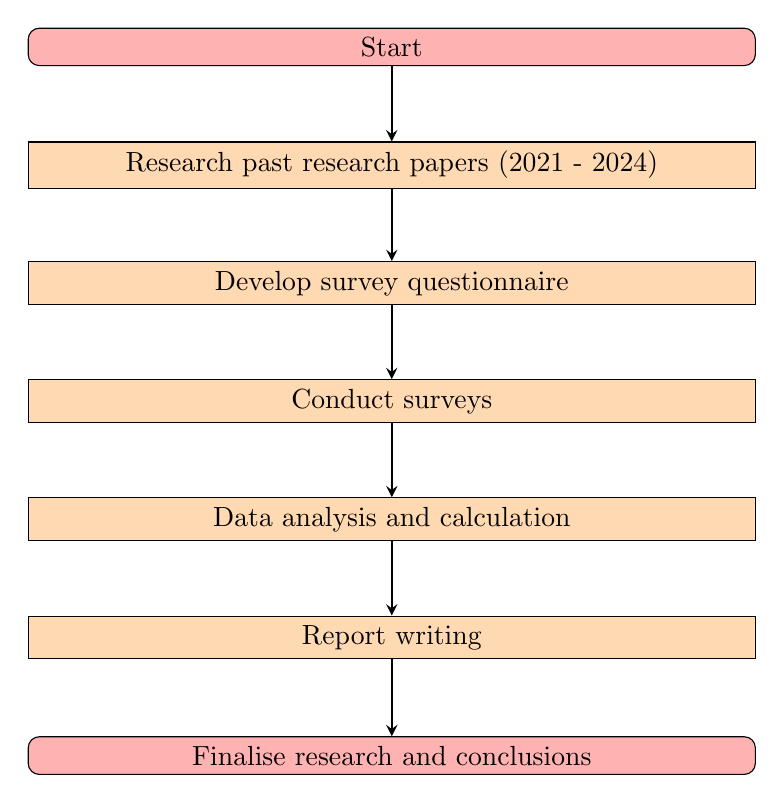
\begin{tikzpicture}[node distance=1.5cm]

        % Nodes
        \node (start) [startstop2] {Start};
        
        \node (pro1) [process2, below of=start] {Research past research papers (2021 - 2024)};
        
        \node (pro2) [process2, below of=pro1] {Develop survey questionnaire};
        
        \node (pro3) [process2, below of=pro2] {Conduct surveys};
        
        \node (pro4) [process2, below of=pro3] {Data analysis and calculation};
        
        \node (end) [process2, below of=pro4] {Report writing};
        
        \node (final) [startstop2, below of=end] {Finalise research and conclusions};

        % Arrows
        \draw [arrow] (start) -- (pro1);
        \draw [arrow] (pro1) -- (pro2);
        \draw [arrow] (pro2) -- (pro3);
        \draw [arrow] (pro3) -- (pro4);
        \draw [arrow] (pro4) -- (end);
        \draw [arrow] (end) -- (final);

    \end{tikzpicture}
    \caption{Research Activity Flowchart}
\end{figure}
\subsection{Milestones}
\begin{table}[H]

\begin{tabular}{|p{3cm}|c|c|c|c|c|c|c|c|}
    \hline
    \textbf{Project Milestones}       & \textbf{Duration (Weeks)} & \textbf{Week 1} & \textbf{Week 2} & \textbf{Week 3} & \textbf{Week 4} & \textbf{Week 5} & \textbf{Week 6} & \textbf{Week 7} \\ 
    \hline
    Identifying the research problem   & 1 & \cellcolor{gray!30} & & & & & & \\ 
    \hline
    Formulating Research Questions and Hypotheses & 1 & & \cellcolor{gray!30} & & & & & \\ 
    \hline
    Research past research papers (2021 - 2024) & 1 & & & \cellcolor{gray!30} & & & & \\
    \hline
    Develop survey questionnaire       & 1 & & & & \cellcolor{gray!30} & & & \\ 
    \hline
    Conduct surveys                    & 1 & & & & & \cellcolor{gray!30} & & \\ 
    \hline
    Data analysis and calculation      & 2 & & & & & \cellcolor{gray!30} & \cellcolor{gray!30} & \\ 
    \hline
    Conclusion                         & 1 & & & & & & \cellcolor{gray!30} & \\ 
    \hline
    Report writing                     & 1 & & & & & & & \cellcolor{gray!30} \\ 
    \hline
\end{tabular}
\centering
\caption{Project Milestones and Timeline (in Weeks)}
\end{table}

\section{Expected Results and Impact}
\subsection{Expected Results}
Given the challenges identified in the Problem Statement, we expect the results of this study to shed light on both the limitations and potential of blockchain technology in the higher education sector. Specifically, we anticipate:
\begin{itemize}
    \item An improved understanding of how blockchain can act as a reliable system for recording certifications, while also revealing key vulnerabilities in cases of erroneous entries. We expect that institutions will highlight the difficulty in correcting data without undermining the integrity of the blockchain.
    \item Insights into how blockchain's reliance on third parties for ledger maintenance raises concerns about privacy and security in handling sensitive student data. Educational institutions are expected to express concerns regarding data exposure and the legal ramifications of such risks.
    \item A cost-benefit analysis on the use of blockchain's energy-intensive validation methods, particularly with respect to long-term sustainability and operational efficiency in educational institutions. We expect to find that, despite its advantages, the use of blockchain might not be economically feasible for many institutions due to its energy consumption.
\end{itemize}
\subsection{Impact}
The findings of this research could have significant implications for both the adoption of blockchain technology in education and its regulatory framework. Based on the results, we expect the following impacts:
\begin{itemize}
    \item \textbf{For Educational Institutions:} The research may lead to a re-evaluation of current data management systems, encouraging the adoption of blockchain for secure, immutable record-keeping, particularly for certification and degree verification. However, institutions may need to reconsider their privacy protocols due to the inherent challenges of third-party reliance.
    \item \textbf{Policy and Regulation:} This research could influence policymakers to design stricter regulations regarding the management of sensitive educational data within blockchain networks. Regulatory bodies may need to consider amendments in privacy laws to ensure students' information is not exposed to unauthorized entities.
    \item \textbf{Technological Innovation:} The study could promote innovations aimed at mitigating blockchain's energy consumption by introducing more eco-friendly alternatives like proof-of-stake systems or hybrid blockchain solutions tailored for the education sector.
    \item \textbf{Cost and Operational Efficiency:} Institutions may weigh the benefits of blockchain against the potential financial burden of maintaining such an infrastructure, influencing future investments in educational technology.
\end{itemize}
Overall, this research will provide a foundation for future studies exploring sustainable, secure, and privacy-compliant applications of blockchain in higher education.

%References
\bibliographystyle{apacite}
\bibliography{MyBib}{}


\end{document}

